%!TEX root = ../Main.tex
\chapter{The system}
\section{The syntax}
The first step to implementing physical space into multi agent systems is having a syntax to express our systems. We will explain the syntax with the support of a step by step example for clarification. 
\begin{table}[H]
\centering
\begin{tabular}{|l l l|} 
 \hline
 Systems & $S ::=$ & $  \Gamma : P\quad |\quad S_1 \ || \ S_2$\\
 Environment & $\Gamma :: =$ & $ \langle \gamma : \mathcal{X} \to \mathcal{V},\quad \mathsf{LS} \rangle $ \\ 
 Processes & $P::=$ & $  0\quad  |\quad  \Pi ! (\Tilde{E})^{E}.U\quad  |\quad  \Pi ? (\Tilde{x})^{E}.U\quad  |\quad \mathsf{S}(\Tilde{E})^{E}.U \quad  |$ \\
 & & $\Pi \mathsf{G}(\Tilde{x})^E.U\quad  |\quad \langle \Pi \rangle P\quad |\quad  P_1 + P_2\quad  |\quad  K(x_1,...,x_n)$\\
 Updates & $U::= $ & $ U[\Tilde{E}/\Tilde{x}]\quad |\quad P\quad |\quad \{\texttt{OP}(\mathsf{LS})\}U$ \\
 Expressions & $E::=$ & $ v\quad |\quad x\quad |\quad ch\quad |\quad self.x\quad |\quad E_1\otimes E_2$ \\[1ex] 
 \hline
\end{tabular}
\caption{The syntax of our calculus.}
\label{Synt}
\end{table}
At the top level we can see the systems $S$. A system is either a process with an environment or a parallel composition of two systems, $S_1\ ||\ S_2$. The environment of a process, $\Gamma$, consists of two things. The first one is $\gamma$, with the form $\mathcal{X} \to \mathcal{V}$, a set of attributes mapped to a set of values of any format. The second one is $\mathsf{LS}$, a set of channels the process is listening to. We will explain more about the properties and function over this set later on in this section.\\
Now that we have gone over the top layer of our syntax, we will present the setup for our example. We will mention the channels, but will go further into how the different types of channels work later on.
\begin{example}\label{ex1}[Product fetching (step 1/5)]
    For our example, we will take a simple setup to make it clear how the channeled communication works. Imagine a warehouse where certain products will have to be collected. Before sending a system to collect the product, it will have to be checked if the needed product is available. If the inventory is available, a manager will have to instruct a worker to fetch the requires product. If the product is unavailable it will have to be refilled. In this section we will not focus on the case of it being empty for simplicity reasons. Later in the thesis we will present the example in full, but as the purpose now is to show how the transitions and examples would look on a process and on a system level, we will keep it simplistic. It will still include all three kinds of communication, namely: broadcast, multicast and unicast. The example will build itself up from the composition, to the specifications, to the process level transitions and finally to the system level transitions. We add the joining and leaving of channels when location comes into play. For now all the processes already have the necessary process in their environment.
\end{example}

As can be seen in \ref{Synt}, a process can take 8 different forms. The first form is the empty process. As the name suggests, this is a process without any function and therefore will stay an empty process. At first glance it might seem useless, but this is very useful as it means we can terminate a process after it has done its part. The process being empty does not mean that the environment is empty, however we will not be able to access this environment anymore.\\
Before we go over the other processes, we will look at their building blocks. Starting with the predicate $\Pi$, which can either evaluate to $True$ or $False$. It is a logical expression over the environment, and can include the basic logical boolean operators. Only processes satisfying the predicate will be able to receive a message or perform their action.\\
An expression $E$ can be a value, an attribute or a channel. It can also include a pointer to an attribute in its own environment, $self.x$, or consists of an operation over expressions. $\Tilde{E}$ presents a sequence of one or more expressions, allowing for passing multiple values. With these clarifications, we will first go over the last 3 process expressions. \\
We have a guarded process $\langle \Pi \rangle P$, this process has an internal guard. It can only continue with the process $P$ if $\Pi$ is satisfied in its own environment. As we do not have parallel process in our syntax, when $\langle \Pi \rangle P$ and $\Pi = False$ under gamma, the process will be blocked for the remainder of the runtime, unless there is a non-syntax related cause, for example it will have to be charged until a certain percentage. Our focus is more on the interaction of processes, and for that where a guard can be helpful is if you want an internal value to determine the next action, which brings us to our next process form.\\
The summation, or $P_1+P_2$, here the process will either continue with $P_1$ or $P_2$, but not both. This choice can be non-deterministic and the non-performed process will be dropped, but more on that later. Combining this with the guarded process can allow us to influence which process will be continued with based on the internal environment. We will also use this in our example later on.\\
The definition process, $K(x_1,...,x_n)$, is a process with its defined attributes. By having this in our syntax, we can express what attributes a process has and where this is internally. Note that for attributes, we cannot have duplicated or the pointers would get messed up. This means we require $x_i\not = x_j iff i\not = j$ for all $1\leq i,j \leq n$.\\
\\
For evaluating $\Pi$ under the environment there are two possible notations. The standard one $\gamma \models \{ \Pi \}_{\gamma}$, which takes the current environment and determines if the predicate holds in that environment. The other notation is $\gamma \models \{ \Pi [\Tilde{v}/ \Tilde{x}] \}_{\gamma}$, this means the predicate should hold with the newly received information. $[\Tilde{v}/ \Tilde{x}]$ stands for substituting the value of $x$ with the corresponding $v$ for each value and attribute in the sequences.\\

\begin{example}\label{ex2}[Product fetching (step 1/5)]
    Our system $S$ consists of 4 processes and can be defined as $S\triangleq C\ ||\ I\ ||\ O\ ||\ R$. Here we have $C$ which checks the inventory with $I$ and then sends the request on to $O$, which orders $R$ to retrieve the desired product. 
\end{example}

This brings us to the communication processes. We will start with the standard send and receive processes, which cover broadcast and multicast, and then cover the get and supply processes of unicast.\\
To begin $\Pi ! (\Tilde{E})^{E}.U$, the sending process. Here $\Pi$ is not an internal guard but rather a predicate for which processes should be able to receive the message. It will be concertized under the environment as $\{ \Pi \}_{\gamma} = \pi'$ and this predicate will be sent along with the message. $\pi '$ only depends on the current values in the receiving process, think of example, their role, battery level, or anything else which can determine if the process should receive the message. The sending process will evaluate the expression $\Tilde{E}$ to $\Tilde{v}$, the values to send, and also the expression $E$ to $ch$, for which channel it will send on. Note that this is not a sequence, so a message can only be sent on a single channel at a time. After sending it will proceed to update its environment about which we will give more details later on what this means.\\
Now for the other end of this interaction, the receiving process $\Pi ? (\Tilde{x})^{E}.U$. Here $\Pi$ is different from $\pi '$, which the process will receive with the message. This guard is of the earlier explained form $\{ \Pi [\Tilde{v}/ \Tilde{x}] \}_{\gamma}$. Both $\Pi$ and $\pi '$ will have to be satisfied in the environment for the process to be able to receive the information. As we can see by $\Tilde{x}$, when a process is expecting a message, it is expecting values for certain attributes. Meaning it is important the combination of the two guards make sure a message only reaches certain processes. This however, is about the specification, not the syntax itself, and differs per setting. After receiving the values, the process will update its current attributes with the received values.\\
The send and receive actions can be done on either broadcast or unicast. As the name suggests, broadcast means all processes will get the message as the broadcast channel $*$, is always in $\mathsf{LS}$. if $ch \not = *$, we are dealing with unicast. Only processes with $ch \in \mathsf{LS}$ will receive this message, but this can still be multiple processes.\\
For unicast we have the process requesting to get information, $\Pi \mathsf{G}(\Tilde{x})^E.U$. We have $\Pi$, which is the same as $\Pi$ in the sending process and is concertized to $\pi '$ and sent along with the request. It sends a sequence of attributes it would like the values of over the channel evaluated from $E$. After receiving the requested information, it updates its attributes with the received values, like the previous receiving process.\\
The get request from the previous process is answered by the supply process, $\mathsf{S}(\Tilde{E})^{E}.U$. As you can see it does not have a guard or predicate, but it still has to satisfy $\pi '$. The reason this process does not have its own guard is that it is not receiving any values to substitute like the receiving process and as it is answering a request, it does not have to send a predicate with its message, like the send and get processes do. The process evaluates $\Tilde{E}$ in accordance to the requested attribute values and sends them back over the same channel, which can be evaluated from $E$. It then performs any internal updates, but these are not necessarily based on the sent information.\\
\\
Now that we have explained the syntax, we can specify the process from our example.
\begin{example}\label{ex3}[Product fetching (step 3/5)] 
    Here are the specifications of the processes in \ref{ex2}.\\
    \begin{table}[H]
    \centering
    \begin{tabular}{l l} 
    $C\triangleq$&$(product=2)G(x)^{self.id}.[self.available := x]$\\
    &$\bigl( \langle self.available \geq 1 \rangle (role="manager")!("start", 2)^*.0+ \langle self.available < 1 \rangle u.0 \bigr)$\\
    $I\triangleq$&$ S(self.inventory)^{self.ch}.[self.inventory:=self.inventory-1].I$\\
    $O\triangleq $&$ (x="start")?(x,y)^*.[self.product:=y]$\\
    & $(status=0,role="receiver")!(self.product)^{self.id}.O$\\
    $R\triangleq $&$ (x=1)?(x)^{self.ch}.[self.product:=x, self.status:=1]p_1\quad + $\\
    &$(x=2)?(x)^{self.ch}.[self.product:=x, self.status:=1]p_2\quad +$ \\
    &$(x=3)?(x)^{self.ch}.[self.product:=x, self.status:=1]p_3$\\
    \end{tabular}
    \label{Syntax}
    \end{table}
\end{example}
We can see that we have some attributes, which we will explain. $id$ is the id of a process and is unique. $product$ is the number of the requested product. $available$ is the number of products of the requested product currently available. $role$ is the role of a process and is can be \textit{manager,receiver,commander,inventory}. $inventory$ is the current inventory size observed, which is the local name of $available$. $Status$ is the status of the process which is either 0 or 1, for busy or not busy. $ch$ is the current channel a process is on and should be in $ch$.

\section{The semantics}
Now that we have our syntax down, we can move on to the rules, or the semantics. We will go over process level semantics first, where the transitions are noted by $\xmapsto[]{}$. Here the possible transition labels are $\lambda$, the send, receive, get and supply transitions.\\
\begin{center}
$\lambda ::=$ $  \Pi ! (\Tilde{v})^{ch}\quad  |\quad \Pi ? (\Tilde{v})^{ch}\quad |\quad \Pi \mathsf{G}(\Tilde{v})^{ch}\quad |\quad \Pi \mathsf{S}(\Tilde{v})^{ch}$
\end{center}
The discard transition, only possible on the receive transition is denoted by $\widetilde{\Pi ? (\Tilde{v})^{ch}}$, in the rule naming this will be denoted by an N in front of the name.

\begin{table}[H]
\small
\centering
\begin{flalign*}
   \texttt{Snd }&\frac{\llbracket \Tilde{E} \rrbracket_\gamma = \Tilde{v}\quad \{\Pi\}_\gamma =\pi '\quad \llbracket E' \rrbracket _\gamma = ch}{\langle \gamma , \mathsf{LS} \rangle : \Pi ! (\Tilde{E})^{E'}.U\xmapsto[]{\pi '! (\Tilde{v})^{ch}} \llbrace \langle \gamma , \mathsf{LS}\rangle : U\rrbrace}& \texttt{Nsnd }&\frac{}{\langle \gamma , \mathsf{LS} \rangle : \Pi ! (\Tilde{E})^{E'}.U\xmapsto[]{\widetilde{\pi '? (\Tilde{v})^{ch}}} \langle \gamma , \mathsf{LS} \rangle : \Pi ! (\Tilde{E})^{E'}.U}\\
   \texttt{Rec }&\frac{\llbracket E ' \rrbracket_\gamma = ch\quad \gamma \models \{\Pi[\Tilde{v}/\Tilde{x}]\} _\gamma\quad \gamma \models \pi ' \quad ch \in \mathsf{LS} }{\langle \gamma , \mathsf{LS} \rangle : \Pi ? (\Tilde{x})^{E'}.U\xmapsto[]{\pi '? (\Tilde{v})^{ch}} \llbrace \langle \gamma , \mathsf{LS}\rangle : U[\Tilde{v}/\Tilde{x}]\rrbrace}&\texttt{Nrec }&\frac{ch \not\in \mathsf{LS} \ \lor \ \bigl(ch = * \ \land \ (\gamma \not\models \{ \Pi [\Tilde{v}/\Tilde{x}]\} \ \lor \ \gamma \not\models \pi ')\bigr)}{\langle \gamma , \mathsf{LS} \rangle : \Pi ? (\Tilde{x})^{E'}.U\xmapsto[]{\widetilde{\pi '? (\Tilde{v})^{ch}}} \langle \gamma , \mathsf{LS} \rangle : \Pi ? (\Tilde{x})^{E'}.U} \\
   \texttt{Get }&\frac{\llbracket E \rrbracket_\gamma = ch\quad \{\Pi\}_\gamma =\pi '}{\langle \gamma , \mathsf{LS} \rangle : \Pi \mathsf{G}(\Tilde{x})^E.U\xmapsto[]{\pi ' \mathsf{G}(\Tilde{v})^{ch}} \llbrace \langle \gamma , \mathsf{LS}\rangle : U[\Tilde{v}/\Tilde{x}]\rrbrace} &\texttt{Nget } &\frac{}{\langle \gamma , \mathsf{LS} \rangle : \Pi \mathsf{G}(\Tilde{x})^E.U\xmapsto[]{\widetilde{\pi ' ? (\Tilde{v})^{ch}}} \langle \gamma , \mathsf{LS} \rangle : \Pi \mathsf{G}(\Tilde{x})^E.U} & \\
   \texttt{Sup }& \frac{\llbracket \Tilde{E} \rrbracket_\gamma = \Tilde{v}\quad \llbracket E' \rrbracket_\gamma = ch\quad \gamma \models \pi '\quad ch\in \mathsf{LS}}{\langle \gamma , \mathsf{LS} \rangle : \mathsf{S}(\Tilde{E})^{E'}.U\xmapsto[]{\pi ' \mathsf{S}(\Tilde{v})^{ch}} \llbrace \langle \gamma , \mathsf{LS}\rangle : U\rrbrace} &\texttt{Nsup } &\frac{ch\not\in \mathsf{LS}\ \lor \ ch = * }{\langle \gamma , \mathsf{LS} \rangle : \mathsf{S}(\Tilde{E})^{E'}.U\xmapsto[]{\widetilde{\pi ' ? (\Tilde{v})^{ch}}} \langle \gamma , \mathsf{LS} \rangle : \mathsf{S}(\Tilde{E})^{E'}.U} & \\
   \texttt{Grd }&\frac{\gamma \models \Pi \quad \langle \gamma , \mathsf{LS}\rangle : P \xmapsto[]{\lambda} \langle \gamma ' , \mathsf{LS} ' \rangle : P'}{\langle \gamma , \mathsf{LS} \rangle : \langle \Pi \rangle P \xmapsto[]{\lambda}\langle \gamma ' , \mathsf{LS} ' \rangle : P'}&\texttt{Blk } &\frac{\gamma \not\models \Pi}{\langle \gamma , \mathsf{LS} \rangle : \langle \Pi \rangle P \xmapsto[]{\widetilde{\pi ' ? (\Tilde{v})^{ch}}}\langle \gamma , \mathsf{LS} \rangle : \langle \Pi \rangle P}\\
   \texttt{Stc }&\frac{\gamma \models \Pi \quad \langle \gamma , \mathsf{LS} \rangle : P \xmapsto[]{\widetilde{\pi ' ? (\Tilde{v})^{ch}}}\langle \gamma , \mathsf{LS} \rangle : P }{\langle \gamma , \mathsf{LS} \rangle : \langle \Pi \rangle P \xmapsto[]{\widetilde{\pi ' ? (\Tilde{v})^{ch}}}\langle \gamma , \mathsf{LS} \rangle : \langle \Pi \rangle P}& &\\
\end{flalign*}
\caption{The process level semantics 1/2.}
\label{opsem1}
\end{table}

We can see that certain rules can always be performed. Either because they only evaluate something or because they have no conditions. These are \texttt{Snd}, \texttt{Nsnd}, \texttt{Get}, \texttt{Nget}. For \texttt{Snd} and \texttt{Get} the reason is that when a process is ready to send or request information, it means it is already able to do this and should proceed when possible. This also means they are not expecting to receive anything and should be able to discard any incoming messages, hence \texttt{Nsnd} and \texttt{Nget}. This has to do with non-blocking behavior and we will go more in dept on that later on in our lemmas.\\
As previously explained for receiving a message through \texttt{Rec} or \texttt{Sup} we have some conditions to be able to receive it. If these do not hold however, we cannot discard the incoming message like for the previous two cases. As we can see one of the conditions is that a process is not listening to a certain channel, which would means they will not even be aware of the message. The other possible condition for discarding a message requires it to be over the broadcast channel. This has to do with the blocking of multicast and unicast, which we will show later in our lemmas. The reason for this blocking behavior is that we do not want processes to be on a non-broadcast channel unless they are participating and ready to continue to the next step.\\
The guard works like explained before, where the condition of discarding in \texttt{Stc} shows that it is only possible when the process is ready and can discard, however if the internal guard does not hold, \texttt{Blk} shows it can discard either way. The example of charging comes to mind, where we do not want a charging process to block.\\
From the rules it shows that after performing an action, it can update its environment with $\llbrace A \rrbrace$. \\
\\
The update function $\llbrace A \rrbrace$ is of the following form:\\
$\llbrace A \rrbrace =
\begin{cases}
\llbrace \langle \gamma [\Tilde{x} \xmapsto[]{} \llbracket \Tilde{E} \rrbracket _\gamma] , \mathsf{LS} \rangle : U \rrbrace, & A=\langle \gamma , \mathsf{LS} \rangle : U[\Tilde{v}/\Tilde{x}]\\
\llbrace \langle \gamma , \texttt{OP}(\mathsf{LS}) \rangle :U \rrbrace, & A=\langle \gamma , \mathsf{LS} \rangle : \{ \texttt{OP}(\mathsf{LS}) \} U \\
\langle \gamma, \mathsf{LS} \rangle : P & A=\langle \gamma, \mathsf{LS} \rangle : P
\end{cases}$
\\
The operation \texttt{OP}($\mathsf{LS}$) on the set of listening channels, can add or remove channels from this set, but $\mathsf{LS}$ will always include the broadcast channel $*$.\\
\begin{table}[H]
\small
\centering
\begin{flalign*}
   \texttt{Lor }&\frac{\langle \gamma , \mathsf{LS} \rangle : P_1 \xmapsto[]{\lambda}\langle \gamma ' , \mathsf{LS}' \rangle : P_1' }{\langle \gamma , \mathsf{LS} \rangle : P_1 + P_2 \xmapsto[]{\lambda}\langle \gamma ' , \mathsf{LS}' \rangle : P_1' } &\texttt{Ror } &\frac{\langle \gamma , \mathsf{LS} \rangle : P_2 \xmapsto[]{\lambda}\langle \gamma ' , \mathsf{LS}' \rangle : P_2' }{\langle \gamma , \mathsf{LS} \rangle : P_1 + P_2 \xmapsto[]{\lambda}\langle \gamma ' , \mathsf{LS}' \rangle : P_2' }\\
   \texttt{Nor }&\frac{\langle \gamma , \mathsf{LS} \rangle : P_1 \xmapsto[]{\widetilde{\pi ' ? (\Tilde{v})^{ch}}}\langle \gamma  , \mathsf{LS} \rangle : P_1 \quad \langle \gamma , \mathsf{LS} \rangle : P_2 \xmapsto[]{\widetilde{\pi ' ? (\Tilde{v})^{ch}}}\langle \gamma  , \mathsf{LS} \rangle : P_2 }{\langle \gamma , \mathsf{LS} \rangle : P_1 + P_2 \xmapsto[]{\widetilde{\pi ' ? (\Tilde{v})^{ch}}}\langle \gamma  , \mathsf{LS} \rangle : P_1 + P_2 } &\\
   \texttt{Def }&\frac{\langle \gamma , \mathsf{LS} \rangle : P \xmapsto[]{\lambda} \langle \gamma ', \mathsf{LS} '\rangle  : P' \quad K(\Tilde{x}) \triangleq P}{\langle \gamma , \mathsf{LS} \rangle : K(\Tilde{x}) \xmapsto[]{\lambda} \langle \gamma ' , \mathsf{LS}' \rangle : P'} &\texttt{Ndef } &\frac{\langle \gamma , \mathsf{LS} \rangle : P \xmapsto[]{\widetilde{\pi ' ? (\Tilde{v})^{ch}}} \langle \gamma , \mathsf{LS} \rangle : P \quad K(\Tilde{x}) \triangleq P}{\langle \gamma , \mathsf{LS} \rangle : K(\Tilde{x}) \xmapsto[]{\widetilde{\pi ' ? (\Tilde{v})^{ch}}} \langle \gamma , \mathsf{LS} \rangle  : P} &\\
   & &\texttt{Nnul }&\frac{}{\langle \gamma , \mathsf{LS}\rangle : 0 \xmapsto[]{\widetilde{\pi ' ? (\Tilde{v})^{ch}}} \langle \gamma , \mathsf{LS}\rangle : 0} &\\
\end{flalign*}
\caption{The process level semantics 2/2.}
\label{opsem2}
\end{table}
The other half of the semantics show how the different cases of the summation notation work, it shows that the 0 process will never be blocking and that the definition process can be treated like any other process.
\begin{example}\label{ex4}[Product fetching (step 4/5)] 
    We can now look at the process level transitions from our example. The environments are as follows:\\
    $\Gamma_C=\langle \gamma : {id=1, product=2, available=0, role="commander", ch=this.id}, \mathsf{LS} ={*, 1}\rangle$\\
    $\Gamma_I=\langle \gamma : {id=2, product=2, available=4, role="inventory", ch=1}, \mathsf{LS} ={*, 1}\rangle$\\
    $\Gamma_O=\langle \gamma : {id=3, product=0, role="manager", ch=self.id}, \mathsf{LS} ={*, 3}\rangle$\\
    $\Gamma_R=\langle \gamma : {id=4, product=0, status=0, role="receiver", ch=3}, \mathsf{LS} ={*, 3}\rangle$\\
    We get the following transitions in order, with $U_i$ being the continuation of the specification of $i$:\\
    $\langle \gamma_C , \mathsf{LS}_C \rangle : C \xmapsto[]{(product=2) \mathsf{G}(4)^1} \llbrace \langle \gamma_C ' , \mathsf{LS}_C ' \rangle : [self.available := x] U_C\rrbrace$ by \texttt{Get}\\
    $\langle \gamma_I , \mathsf{LS}_I \rangle : I \xmapsto[]{(product=2) \mathsf{S}(4)^1} \llbrace \langle \gamma_I ' , \mathsf{LS}_I ' \rangle : [self.inventory:=self.inventory-1].I\rrbrace$ by \texttt{Sup}\\
    $\langle \gamma_C ' , \mathsf{LS}_C ' \rangle : U_C \xmapsto[]{(role="manager")! ("start", 2)^*} \llbrace \langle \gamma_C '' , \mathsf{LS}_C '' \rangle : 0\rrbrace$ by \texttt{Lor}\\
    $\langle \gamma_O , \mathsf{LS}_O \rangle : O \xmapsto[]{(role="manager")? ("start", 2)^*} \llbrace \langle \gamma_O ' , \mathsf{LS}_O ' \rangle : [self.product:=2].U_O\rrbrace$ by \texttt{Rec}\\
    $\langle \gamma_I ' , \mathsf{LS}_I ' \rangle : I \xmapsto[]{\widetilde{(role="manager")? ("start", 2)^*}} \langle \gamma_I ' , \mathsf{LS}_I ' \rangle : I$ by \texttt{Nrec}\\
    $\langle \gamma_R , \mathsf{LS}_R \rangle : R \xmapsto[]{\widetilde{(role="manager")? ("start", 2)^*}} \langle \gamma_R , \mathsf{LS}_R \rangle : R$ by \texttt{Nrec}\\
    $\langle \gamma_O ' , \mathsf{LS}_O ' \rangle : U_O \xmapsto[]{(status=0,role="receiver")!(2)^{3}} \llbrace \langle \gamma_O '' , \mathsf{LS}_O '' \rangle : O\rrbrace$ by \texttt{Snd}\\
    $\langle \gamma_R , \mathsf{LS}_R \rangle : R \xmapsto[]{(status=0,role="receiver")!(2)^{3}} \llbrace \langle \gamma_R ' , \mathsf{LS}_R ' \rangle : [self.product:=2, self.status:=1]p_2\rrbrace$ by \texttt{Lor}, \texttt{Ror} and \texttt{Rec}\\
\end{example}
For the system level we introduce one more transition label, the unicast transition $\tau$. For the possible transition labels we then have:\\
\begin{center}
$ \alpha ::=\quad \lambda \quad |\quad \tau$\\
\end{center}
We can then define the following system level semantics:
\begin{table}[H]
\normalsize
\centering
\begin{flalign*}
    \texttt{Sys }&\frac{\langle \gamma, \mathsf{LS}\rangle : P \xmapsto[]{\lambda}\langle \gamma ', \mathsf{LS} ' \rangle : P' }{\langle \gamma, \mathsf{LS}\rangle : P \xrightarrow[]{\lambda}\langle \gamma ', \mathsf{LS} ' \rangle : P'} &\texttt{Nsys } &\frac{\langle \gamma, \mathsf{LS}\rangle : P \xmapsto[]{\widetilde{\Pi ? (\Tilde{v})^{ch}}}\langle \gamma , \mathsf{LS} \rangle : P }{\langle \gamma, \mathsf{LS}\rangle : P \xrightarrow[]{\Pi ? (\Tilde{v})^{ch}}\langle \gamma , \mathsf{LS} \rangle : P} &\\
    \texttt{Prec }&\frac{S_1 \xrightarrow[]{\Pi ? (\Tilde{v})^{ch}} S_1' \quad S_2 \xrightarrow[]{\Pi ? (\Tilde{v})^{ch}} S_2'}{S_1 \ || \ S_2 \xrightarrow[]{\Pi ? (\Tilde{v})^{ch}} S_1 ' \ || \ S_2' } & & &\\
    \texttt{Lpar }&\frac{S_1 \xrightarrow[]{\Pi ! (\Tilde{v})^{ch}} S_1'\quad S_2 \xrightarrow[]{\Pi ? (\Tilde{v})^{ch}} S_2'}{S_1 \ || \ S_2 \xrightarrow[]{\Pi ! (\Tilde{v})^{ch}} S_1' \ || \ S_2'} &\texttt{Rpar } &\frac{S_1 \xrightarrow[]{\Pi ? (\Tilde{v})^{ch}} S_1'\quad S_2 \xrightarrow[]{\Pi ! (\Tilde{v})^{ch}} S_2'}{S_1 \ || \ S_2 \xrightarrow[]{\Pi ! (\Tilde{v})^{ch}} S_1' \ || \ S_2' } &\\
    \texttt{Lsup }&\frac{S_1 \xrightarrow[]{\Pi \mathsf{S} (\Tilde{v})^{ch}} S_1' }{S_1 \ || \ S_2 \xrightarrow[]{\Pi \mathsf{S} (\Tilde{v})^{ch}} S_1 ' \ || \ S_2 } &\texttt{Rsup } &\frac{S_2 \xrightarrow[]{\Pi \mathsf{S} (\Tilde{v})^{ch}} S_2' }{S_1 \ || \ S_2 \xrightarrow[]{\Pi \mathsf{S} (\Tilde{v})^{ch}} S_1  \ || \ S_2' } & \\
    \texttt{Lget }&\frac{S_1 \xrightarrow[]{\Pi \mathsf{G} (\Tilde{v})^{ch}} S_1' }{S_1 \ || \ S_2 \xrightarrow[]{\Pi \mathsf{G} (\Tilde{v})^{ch}} S_1 ' \ || \ S_2 } &\texttt{Rget } &\frac{S_2 \xrightarrow[]{\Pi \mathsf{G} (\Tilde{v})^{ch}} S_2' }{S_1 \ || \ S_2 \xrightarrow[]{\Pi \mathsf{G} (\Tilde{v})^{ch}} S_1  \ || \ S_2' } & \\
    \texttt{Luni }&\frac{S_1 \xrightarrow[]{\Pi \mathsf{G} (\Tilde{v})^{ch}} S_1'\quad S_2 \xrightarrow[]{\Pi \mathsf{S} (\Tilde{v})^{ch}} S_2'}{S_1 \ || \ S_2 \xrightarrow[]{\tau} S_1' \ || \ S_2'} &\texttt{Runi } &\frac{S_1 \xrightarrow[]{\Pi \mathsf{S} (\Tilde{v})^{ch}} S_1'\quad S_2 \xrightarrow[]{\Pi \mathsf{G} (\Tilde{v})^{ch}} S_2'}{S_1 \ || \ S_2 \xrightarrow[]{\tau} S_1' \ || \ S_2'} & \\
    \texttt{Ltau }&\frac{S_1 \xrightarrow[]{\tau} S_1}{S_1 \ || \ S_2 \xrightarrow[]{\tau} S_1' \ || \ S_2} &\texttt{Rtau } &\frac{S_2 \xrightarrow[]{\tau} S_2'}{S_1 \ || \ S_2 \xrightarrow[]{\tau} S_1 \ || \ S_2'} & \\
\end{flalign*}
\caption{The system level semantics.}
\label{opsem3}
\end{table}
We can see in \ref{opsem3} that on a system level, denoted by $\xrightarrow[]{}$, we cannot see the discard transition. In addition we get a new transition $\tau$, this is also called the hidden transition and it occurs when unicast communication is performed.

\begin{example}\label{ex5}[Product fetching (step 5/5)] 
    We can now look at the system level transitions from our example.\\
    $C\ ||\ I\ ||\ O\ ||\ R \xrightarrow[]{\tau}U_C\ ||\ I'\ ||\ O\ ||\ R$\\
    $U_C\ ||\ I'\ ||\ O\ ||\ R \xrightarrow[]{(role="manager")! ("start", 2)^*}0\ ||\ I'\ ||\ U_O\ ||\ R$\\
    $U_C\ ||\ I'\ ||\ O\ ||\ R \xrightarrow[]{(status=0,role="receiver")!(2)^{3}}0\ ||\ I'\ ||\ O\ ||\ p_2$\\
\end{example}
As we can see this is a lot clearer of an overview. But we do not know what $C$ and $I$ communicated, nor do we know how the environments updated. 
\\
\section{Lemmas}
We will first state some essential lemmas, to prove certain behaviorial properties of our system. The proofs of these lemmas can be found in the appendix.\\
\begin{lemma}
    \begin{enumerate}
    \item $S_1 \ || \ S_2 \equiv S_2\ ||\ S_1$
    \item $(S_1 \ ||\ S_2 )\ || \ S_3 \equiv S_1 \ ||\ (S_2 \ || \ S_3)$
    \item $S_1 \ || \ \Gamma : 0 \equiv S_1$
\end{enumerate}
\end{lemma}
Given 2 systems $S_1$ and $S_2$ proof:
\begin{lemma}
Lemma 2 is regarding the non-blocking behavior of broadcasted messages.\\ 
$ch=* \land S_1 \xrightarrow[]{\pi !(\Tilde{v})^{ch}}S_1' \implies S_1\ ||\ S_2 \xrightarrow[]{\pi !(\Tilde{v})^{ch}}S_1'\ ||\ S_2'\quad $ for any $S_2$.\\
\end{lemma}
\begin{lemma}
    Lemma 3 shows the blocking of multi cast channels.\\
$ch\not = * \land S_1 \xrightarrow[]{\pi !(\Tilde{v})^{ch}}S_1' \implies S_1\ ||\ S_2 \xrightarrow[]{\pi !(\Tilde{v})^{ch}}S_1'\ ||\ S_2'\quad$ for any $S_2$ such that:
\begin{enumerate}
    \item $ch \in \mathsf{LS} \land S_2 \xrightarrow[]{\pi ?(\Tilde{v})^{ch}}S_2'$\\
    $\lor$
    \item $ch \not \in \mathsf{LS}$
\end{enumerate}
\end{lemma}
\begin{lemma}
    This lemma is about the blocking of unicast, to show it should never go unanswered\\
$S_1 \xrightarrow[]{\Pi \mathsf{G} (\Tilde{v})^{ch}} S_1' \implies S_1 \ || \ S_2 \xrightarrow[]{\tau} S_1' \ || \ S_2'$ for any $S_2$ such that $S_2 \xrightarrow[]{\Pi \mathsf{S} (\Tilde{v})^{ch}} S_2'$. 
\end{lemma}
\section{Context}
Now that we have the basis of our model, we can add the reasoning about physical space. For this we will define an other layer to our syntax, the Context layer.\\
\begin{table}[H]
\centering
\begin{tabular}{|l l l|}
 \hline
 Context & $C ::=$ & $  [S]^{\gamma , \mathsf{LS}}\quad |\quad C_1 \ || \ C_2$\\
 \hline
\end{tabular}
\caption{The syntax of our context.}
\label{cont}
\end{table}
A context is a subsection of the physical space in which our system exists. To clarify some of the definition we will use an example space as shown in \ref{fig:examplespace}. This is a simplified layout of a physical space, we will go further into how we can divide and reason about the context for spaces.
\begin{figure}[H] 
		 \centering
		 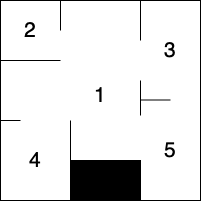
\includegraphics[width=2in]{figure/Map.drawio.png} 
		 \caption{Example of space layout} 
		 \label{fig:examplespace} 
\end{figure}
In Table~\ref{cont} we first have the singular context $[S]^{\gamma , \mathsf{LS}}$. Here the context would be one of the numbered rooms and $S$ would exist in that room. Note that $S$ can be an empty process, in other words, a context does not require a system to be present to exist. We can also see that each context has an environment, just like the systems. $\gamma$ stores the local variables and the physical space representation and $\mathsf{LS}$ stores the local channels. In the semantics we will see how this environment influences the systems present in the context. A context can also be a parallel composition of contexts, these parallel compositions allow for representing a full physical space, without the need for specified relations. For non-continuous, or discrete, space, this can be helpful as we do not have to keep track of the relations between contexts as their relation will no change, but they still exist in parallel. As our example has no defined continuous spaces, here the spaces would exist in parallel.
\\
The other two contexts define the relations between contexts. For this we have two different options, namely the externally connected relation $\mathsf{EC}(C_1, C_2)^{\gamma , \mathsf{LS}}$, this relation argues that systems from 1 context could move to the other context and depending on the specified model, could also communicate between the contexts. Relating it to \ref{fig:examplespace}, we would have $\mathsf{EC}(1,2)$  for example, as space 1 is directly connected to space 2. The environment of this context is a union of the environment of $C_1$ and $C_2$. The opposite of externally connected is disconnected $\mathsf{DC}(C_1, C_2)^{\gamma , \mathsf{LS}}$. As we do not allow for movements to non-externally connected contexts, disconnected contexts limit the possible actions which can be taken. The environment is again a combination of both contexts, and for continuous contexts could be used for moving closer to eventually allow for the exchanging of processes. In relation to \ref{fig:examplespace}, this would be $\mathsf{DC}(2,4)$. We would most likely not define this relation for discrete physical spaces like these rooms, as just saying they exist in parallel also argues that they cannot directly exchange processes.
\\
For our context semantics, to distinguish them from the other transition levels, we will use $\xRightarrow[]{}$ for context level transitions. We will use the transition label $\mu (S, E)$ to model movements, where $S$ is the system which moves and $E$ an expression which can be concretized to a destination context.
\begin{table}[H]
\normalsize
\centering
\begin{flalign*}
    \texttt{Out }&\frac{}{[\langle \gamma _S, \mathsf{LS}_S\rangle : S]^{\gamma _C, \mathsf{LS}_C} \xRightarrow[]{\mu (S, C')}[\quad]^{\gamma _C', \mathsf{LS}_C}} & & &\\
    \texttt{In } &\frac{}{[\quad]^{\gamma _C, \mathsf{LS}_C} \xRightarrow[]{\mu (S, C)}[\langle \gamma _S \cup \gamma _C, \mathsf{LS}_S \cup \mathsf{LS} _C \rangle : S']^{\gamma _C', \mathsf{LS}_C}} & & &\\
   \texttt{LPOut }&\frac{}{[\langle \gamma _{S_1}, \mathsf{LS}_{S_1}\rangle : S_1\ ||\ \langle \gamma _{S_2}, \mathsf{LS}_{S_2}\rangle : S_2]^{\gamma _C, \mathsf{LS}_C} \xRightarrow[]{\mu (S_1, E)}[\langle \gamma _{S_2}, \mathsf{LS}_{S_2}\rangle : S_2]^{\gamma _C', \mathsf{LS}_C}} & & &\\
     \texttt{RPOut }&\frac{}{[\langle \gamma _{S_1}, \mathsf{LS}_{S_1}\rangle : S_1\ ||\ \langle \gamma _{S_2}, \mathsf{LS}_{S_2}\rangle : S_2]^{\gamma _C, \mathsf{LS}_C} \xRightarrow[]{\mu (S_2, E)}[\langle \gamma _{S_1}, \mathsf{LS}_{S_1}\rangle : S_1]^{\gamma _C', \mathsf{LS}_C}} & & &\\
%    \texttt{LPIn } &\frac{}{[\langle \gamma _{S_2}, \mathsf{LS}_{S_2}\rangle : S_2]^{\gamma _C, \mathsf{LS}_C} \xRightarrow[]{\mu (S_1, C)}[\langle \gamma _{S_1} \cup \gamma _C, \mathsf{LS}_{S_1'} \cup \mathsf{LS} _C \rangle : S_1'\ ||\ \langle \gamma _{S_2}, \mathsf{LS}_{S_2}\rangle : S_2]^{\gamma _C', \mathsf{LS}_C}} & & &\\
        \texttt{RPIn } &\frac{}{[\langle \gamma _{S_1}, \mathsf{LS}_{S_1}\rangle : S_1]^{\gamma _C, \mathsf{LS}_C} \xRightarrow[]{\mu (S_2, C)}[\langle \gamma _{S_1}, \mathsf{LS}_{S_1}\rangle : S_1\ ||\ \langle \gamma _{S_2} \cup \gamma _C, \mathsf{LS}_{S_2} \cup \mathsf{LS} _C \rangle : S']^{\gamma _C', \mathsf{LS}_C}} & & &\\
    \texttt{LMov }&\frac{EC(C_1, C_2)}{[\langle \gamma _S, \mathsf{LS} _S \rangle : S]_1^{\gamma _{C_1}, \mathsf{LS}_{C_1}} \ || \ [\quad]_2^{\gamma _{C_2}, \mathsf{LS}_{C_2}} \xRightarrow[]{\mu (S, C_2)} [\quad]_1^{\gamma _{C_1}, \mathsf{LS}_{C_1}} \ || \ [\langle (\gamma _S \setminus \gamma _{C_1})\cup \gamma _{C_2}, (\mathsf{LS} _S \setminus \mathsf{LS} _{C_1}) \cup \mathsf{LS} _{C_2} \rangle : S']_2^{\gamma _{C_2}, \mathsf{LS}_{C_2}}} & & &\\
    \texttt{RMov }&\frac{EC(C_1, C_2)}{[\quad]_1^{\gamma _{C_1}, \mathsf{LS}_{C_1}} \ || \ [\langle \gamma _S, \mathsf{LS} _S \rangle : S]_2^{\gamma _{C_2}, \mathsf{LS}_{C_2}} \xRightarrow[]{\mu (S, C_1)} [\langle (\gamma _S \setminus \gamma _{C_2})\cup \gamma _{C_1}, (\mathsf{LS} _S \setminus \mathsf{LS} _{C_2}) \cup \mathsf{LS} _{C_1} \rangle : S']_1^{\gamma _{C_1}, \mathsf{LS}_{C_1}} \ || \ [\quad]_2^{\gamma _{C_2}, \mathsf{LS}_{C_2}}} & & &\\
%    \texttt{Con }&\frac{}{[S_1]_1^{\gamma _{C_1}, \mathsf{LS}_{C_1}} \ || \ [S_2]_2^{\gamma _{C_2}, \mathsf{LS}_{C_2}} \xRightarrow[]{\mathsf{EC}(C_1, C_2)} [S_1\ ||\ S_2 ]^{\gamma _{C_1} \cup \gamma _{C_2}, \mathsf{LS}_{C_1} \cup \mathsf{LS} _{C_2}}} & & &\\
%    \texttt{Dis }&\frac{}{[S_1\ ||\ S_2 ]^{\gamma _{C_1} \cup \gamma _{C_2}, \mathsf{LS}_{C_1} \cup \mathsf{LS} _{C_2}} \xRightarrow[]{\mathsf{DC}(C_1, C_2)} [S_1]_1^{\gamma _{C_1}, \mathsf{LS}_{C_1}} \ || \ [S_2]_2^{\gamma _{C_2}, \mathsf{LS}_{C_2}}} & & &\\
\end{flalign*}
\caption{The system level semantics.}
\label{opsem4}
\end{table}


